\section{A nerve theorem with constructed homotopies}
\label{sec:boxnerve}

The ProveIt topology report leaves open an effective nerve theorem with
produced contraction data (\href{https://github.com/VladimirReshetnikov/ProveIt/blob/5f3be02388442f16487d2dc5c2529961dd783d2b/Logic/PrimitiveRecursiveArithmetic/docs/proofs/topology/ipra_topology_framework_2026-11-15/paper/sections/12_limits.tex}{topology report, residual obligations}). Here is a case in which the input consists
entirely of coordinates. It includes spaces with holes, disconnected
spaces, boxes of dimension less than the ambient dimension, and
intersections with zero clearance. The classical closed convex nerve
theorem and the forward map from a subdivided nerve are well established
(Bauer, Kerber, Roll and Rolle, \emph{Expositiones Mathematicae}, 2023,
\href{https://doi.org/10.1016/j.exmath.2023.04.005}{doi:10.1016/j.exmath.2023.04.005}).
The issue here is the arithmetic cost of constructing both homotopies,
particularly near a boundary shared by several boxes.

\paragraph{The statement.}
Let $B_1,\ldots,B_m$ be nonempty closed axis-parallel rational boxes in
$\mathbb R^d$, with $m\geq1$. Write $U=\bigcup_i B_i$ and let $N$ have a
nonempty face $J\subseteq\{1,\ldots,m\}$ precisely when
$\bigcap_{i\in J} B_i\ne\varnothing$. Realize $|N|$ in the probability
simplex by requiring the support of a point to be a face. Use the maximum
norm on both spaces. On finite rational data there are primitive recursive
constructions of maps
\[
 F:U\longrightarrow |N|,\qquad G:|N|\longrightarrow U
\]
and homotopies from the identities to $GF$ and $FG$. The constructions
supply rational Lipschitz bounds for every map and homotopy. They extend
to regular Cauchy names. An inclusion of covers taking each box into a specified
target box commutes with $G$ up to a constructed homotopy. An empty
family can be handled separately by the empty nerve and the empty union.

\paragraph{Finite presentations.}
Write $B_i=\prod_j[\ell_{ij},u_{ij}]$. For nonempty $J$, compute
$L_j(J)=\max_{i\in J}\ell_{ij}$ and
$V_j(J)=\min_{i\in J}u_{ij}$. Testing $L_j\leq V_j$ for every $j$
decides the nerve table, including tangencies. A positive result gives
the point $p_J=(L_j(J))_j$ and the contraction to $p_J$ by linear
interpolation in the intersection.

Cut the bounding rectangle $R$ by all box endpoints in each coordinate.
The factors of a grid face are knots or closed intervals between successive
knots. Retain every face $c$ contained in at least one $B_i$. These faces
form a cubical complex $K$ with realization $U$. Indeed each box and all
its faces are unions of grid faces. Set $I(c)=\{i:c\subseteq B_i\}$.
This is a nerve face, since the center of $c$ belongs to all its boxes.
Inclusion of grid faces reverses inclusion of their index sets. The grid
has at most $(4m-1)^d$ nonempty faces before restriction and $N$ has at most
$2^m-1$ nonempty faces. Each coordinate with a single knot is kept constant.

For any nonempty face $J$ of the probability simplex let $b_J$ have value
$1/|J|$ on $J$ and zero elsewhere. Barycentric subdivision of the grid has
a simplex for each strict chain $c_0\subsetneq\cdots\subsetneq c_s$,
with vertices the centers $b(c_j)$ of these faces. To see directly that it
covers a box face, join its center to the subdivision of its boundary.
Every point other than the center lies on a unique radial ray from the
center to that boundary. Repeating on faces gives a convex combination of
centers down to dimension zero. The subdivisions on common faces agree.
For the probability simplex there is an equally explicit description.
Sort the distinct positive coordinate values $v_1>\cdots>v_k>0$, set
$v_{k+1}=0$, and use $J_a=\{i:y_i\geq v_a\}$.
The coefficient of $b_{J_a}$ is $|J_a|(v_a-v_{a+1})$. These nonnegative
coefficients sum to one and telescope in each coordinate.
Coincident values introduce a zero coefficient in a sorted enumeration.
No choice on a shared boundary affects the interpolation.

\paragraph{The two maps.}
On a subdivided grid vertex put $F(b(c))=b_{I(c)}$. Extend affinely along
each chain. Its images are a chain of barycenters of nerve faces in reverse
order, with possible repetitions. Hence $F(x)\in |N|$.
Put $G(b_J)=p_J$ and extend affinely on each subdivided nerve simplex.
For a chain $J_0\subsetneq\cdots\subsetneq J_k$, all its selected points
belong to each $B_i$ for $i\in J_0$. Convexity gives the same containment
for $G(y)$. Affine formulas agree on faces in both constructions.

For $x$ in a grid chain ending at $c_s$, choose any $i\in I(c_s)$.
The point $x$ lies in $B_i$. Every $I(c_j)$ contains $i$, so
$p_{I(c_j)}\in B_i$. Since $G$ is affine on the chain of the $I(c_j)$,
$GF(x)$ is the combination of these latter points with the original
weights. Thus $(1-t)x+tGF(x)$ stays in $B_i$ for $0\leq t\leq1$.

\paragraph{The homotopy on the nerve.}
Fix a rational $y$ with its positive-weight chain
$J_0\subsetneq\cdots\subsetneq J_k$. Choose $i\in J_0$. Every barycenter
in this chain has $i$-coordinate at least $1/m$. Thus $y_i\geq1/m$.
The point $G(y)$ belongs to $B_i$. More generally, whenever $x\in B_i$,
the largest grid face with positive weight in its subdivided presentation
is contained in $B_i$. Indeed $x$ lies in the relative interior of that
face, because its center has positive weight. A box with grid endpoints
containing such a point contains the entire face. Every smaller face
in the chain is contained as well. Consequently $F(x)_i\geq1/m$.
Taking $x=G(y)$ gives a coordinate shared with quantitative mass:
\[
  y_i\geq1/m,\qquad (FG(y))_i\geq1/m.
\]
The calculation of the homotopy does not require the index $i$.
Write $v=FG(y)$ and define
\[
   z_j=\min(y_j,v_j),\qquad S=\sum_j z_j\geq1/m,\qquad P(y)=z/S.
\]
The support of $P(y)$ lies in both supports. Travel along the segment
from $y$ to $P(y)$ during the first half of the unit interval and along
the segment from $P(y)$ to $v$ during the second half. Each segment lies
in a single nerve simplex. The midpoint formulas agree. This construction
gives a global formula using only rational operations and a guarded
reciprocal. It also works when the direct segment from $y$ to $v$ leaves
the nerve.

\paragraph{Continuity and proof strength.}
Here are bounds that do not presume a Lebesgue number for the input.
Extend the vertex formula for $F$ to every grid face in $R$, assigning
$e_1$ whenever $I(c)$ is empty. Extend $G$ to the entire probability
simplex, assigning $p_{\{1\}}$ on barycenters of nonfaces. Their affine
extensions still land in the full simplex and in $R$, respectively.
Compute the affine matrices of the finitely many full-dimensional pieces
by solving their rational vertex equations. Constant domain coordinates
are dropped, and for the probability simplex the last coordinate is
dropped. The latter projection is $1$-Lipschitz into the coordinate
chart with maximum norm. In dimension zero the linear part is zero.
The largest absolute row sum over all pieces is a Lipschitz bound on a
convex domain: a rational segment can be cut at its intersections with
the finite affine walls, and the lengths of its collinear pieces sum to
the segment length. If a segment lies on a wall the two adjacent affine
formulas agree there. Thus the two computed bounds $L_F,L_G$ work even
for pairs lying in distinct components of the original domain.
The determinant algorithm may use the bounded permutation formula.

Set $D=L_FL_G$ and $L=\max(1,D)$. The first homotopy has Lipschitz bound
$L+\operatorname{diam}_\infty R$ on the product with time, using the maximum
product metric. For the second, $z$ is $L$-Lipschitz and $S$ is
$mL$-Lipschitz. Comparing $z_j/S$ with $z'_j/S'$ and using
$z'_j/S'\leq1$ bounds the change by
$m(|z_j-z'_j|+|S-S'|)$. Thus $P$ is $m(1+m)L$-Lipschitz on $|N|$.
Interpolating in time costs at most $2$, so $m(1+m)L+2$ suffices for
the second homotopy. If an evaluator has bound $A$, an input known to
accuracy $2^{-(k+\lceil A\rceil+1)}$ gives output error below $2^{-k}$.
This intentionally coarse shift avoids logarithms.

Internally, use rational points of $U$ and $|N|$ as dense presentations
and code all regular names via their rational observations. An input
approximation on either side is required to belong to the presented
rational space. Rational cell location is decidable, and common-face
agreement and the Lipschitz bounds make the output independent of
approximants. Externally, the resulting maps extend to the metric
completions; in ordinary real geometry these are exactly the indicated
closed polyhedra. This distinction avoids a case decision on an exact
real at a box face. All statements about pointwise errors reduce to
cleared rational inequalities. To implement the two subdivisions,
enumerate chains of length at most $d+1$ for the grid or $m$ for the
nerve, discard dependent candidates by a determinant test and test
barycentric coefficients by sign and summation. Lower-dimensional
chains use any nonsingular minor of the right size and check all ambient
equations. Include the singleton case. All scans are bounded by the
face counts above raised to the corresponding chain lengths, up to
summing over lengths; each coordinate scan and each permutation sum has
its own finite bound. Existence of a containing simplex follows from
the radial decomposition with at most $d$ strict dimension drops or
from the sorted-coordinate formula with at most $m$ steps. At a grid
face $[a,b]$, the radial step divides by the largest of the absolute
rescaled coordinates $|2(x_j-a_j)/(b_j-a_j)-1|$ over nonconstant
coordinates, after testing the center case. Rational comparison guards
this division.

A quantifier-free induction for the weighted-coordinate estimate keeps
a partial numerator and the corresponding sum of weights. The invariant
after $r$ terms is
$m\sum_{j<r}w_j a_j\geq D_0\sum_{j<r}w_j$, where coordinates have
common denominator $D_0$ and $m a_j\geq D_0$. The next inequality follows
by multiplication by $w_r$ and addition. The mass bound uses the
one summand belonging to the common coordinate. Grid tests, incidence
checks, membership of a running intersection, and agreement of two
affine pieces at the vertices of their common face are finite Boolean
folds. On a fixed rational segment the partition at affine walls has
at most two endpoints per simplex in a brute-force implementation:
intersection of a simplex with a line segment is an interval whose
endpoints follow from its rational barycentric inequalities. Sorting
these rational parameters and summing the Lipschitz estimates is
another quantifier-free prefix invariant. The capacity bounds above
are primitive recursive in the input, including the dimension.

\paragraph{Naturality for inclusions and an exact persistence interval.}
Suppose $B_i\subseteq C_{r(i)}$ for a finite index map $r$. Let
$r_*$ send each subdivided vertex $b_J$ to $b_{r(J)}$ and be affine on
chains. Taking images of finite subsets commutes with composition,
including collapsed faces. For $y$ in a chain beginning at $J_0$,
pick $i\in J_0$. Both $G_B(y)$ and $G_C(r_*y)$ are in $C_{r(i)}$.
The straight homotopy in that box proves commutation up to homotopy.
The usual linear nerve map and $r_*$ are likewise joined by straight
segments: on a chain ending at $J_k$ both lie in the simplex $r(J_k)$.
All these arguments work at face contacts.
Consequently in the usual homology interpretation the nerve isomorphisms
respect the maps of a filtration. This uses ordinary homotopy invariance
as a semantic consequence; the finite arithmetic output consists of the
maps, homotopies, and their budgets.

For instance, take the bottom, right, top and left bars
\[
 [0,3]\times[0,1],\quad [2,3]\times[0,3],\quad
 [0,3]\times[2,3],\quad [0,1]\times[0,3]
\]
in that order. At $y=(3/4,1/4,0,0)$ the subdivided weights on
$\{1\},\{1,2\}$ are both $1/2$. Thus $G(y)=(1,0)$,
$FG(y)=(1/2,0,0,1/2)$, $S=1/2$ and $P(y)=e_1$.
The union of the two endpoint supports contains the disjoint left and
right bars. A single straight homotopy between those endpoints would
leave the nerve (Figure~\ref{fig:boxnerve}).
\begin{figure}[htbp]
  \centering
  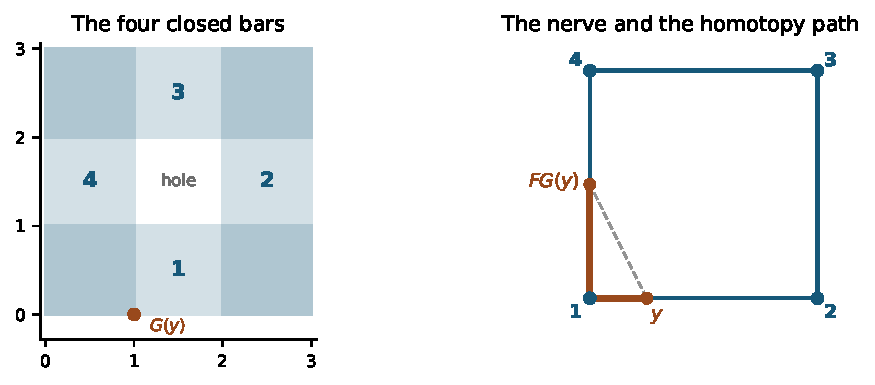
\includegraphics[width=.86\linewidth]{figures/box_nerve.pdf}
  \caption{The four bars and their nerve at $t=0$. The orange path passes
  through vertex $1$. The dashed chord crosses the missing simplex.}
  \label{fig:boxnerve}
\end{figure}
Now thicken all bars in the maximum norm by $t\geq0$.
For $t<1/2$ consecutive bars meet and opposite ones are disjoint, so
the nerve is exactly a four-cycle. For $t\geq1/2$, $(3/2,3/2)$ belongs
to all four, so the nerve is the full tetrahedron. Inclusion before the
threshold induces the identity on the four labels. Over $\mathbb F_2$,
the only nonzero $1$-cycle in the four-cycle is the sum of its four
edges, since even incidence at every vertex forces all coefficients to
coincide. There are no triangles. In the full simplex every $1$-cycle
bounds: cone its edges to vertex $1$, omitting repeated-vertex
triangles; the terms from incident endpoints cancel by even incidence.
Hence this filtration has exactly one degree-one interval $[0,1/2)$.
Rational $t$ already gives its entire finite-arithmetic statement.
The exact evaluator in \texttt{examples/box\_nerve.py} reproduces these
intersections, both maps at the specified point, and the overlap mass.

\paragraph{Lean path.}
\texttt{lean/Topology.lean} proves the intersection fold, lower-corner
criterion, weighted-coordinate lower bound, support of a minimum, and
the overlap denominator estimate after clearing denominators. Its
\texttt{overlap\_segments} theorem constructs the two segments at rational
parameters: blending $x/D$ and $z/S$ with time $b/(a+b)$ gives numerators
$aS x_j+bD z_j$ with total $(a+b)DS$. It proves the corresponding total
and valid support on both halves.
To finish the spatial layer, code an axis face by a knot or an interval
index and use face chains with rational barycentric weights. Prove the
radial-step reconstruction by clearing its tested denominator, then
induct on the number of nonconstant coordinates. Prove reconstruction
of the simplex coordinates by telescoping sorted differences. On these
witnesses the two interpolation maps are finite weighted sums.
Composing the two chain maps on the grid side only merges repeated
index sets, preserving those sums. On the nerve side apply
\texttt{weighted\_lower} twice to the common-index argument and
\texttt{overlap\_mass} once before dividing. The remaining estimates are
the affine matrix calculation and rational segment subdivision above.
Quoting these finite kernels into the repository calculus remains a
separate derivation task. Arbitrary convex bodies given by membership
oracles would require additional procedures for producing their
intersection witnesses and a compatible subdivision.
